% Drawing 74/05-7 -- folder 74, batch 05, archive page 83 (PDF page 84).
% Transcription: Cinq esquisses de pyramides et de bipyramides en perspective (sommets marqués, arêtes croisées), dont deux barrées d'une croix au crayon, et une entourée d'un arc ; à côté, des pointillés.
% Kind: sketches of pyramids and bipyramids. Method 2 (schematic redraw from the facsimile). Status: partial.
% Notes: Five sketches in perspective: three pyramids in the upper row (the second and third barred by a pencil cross), two bipyramids below, the second within an arc; a dotted stroke at the right. Edges approximate (overinked crossings).
% Coordinates: 1 unit = 1 mm = 1/100 of the crop width (bbox in page fractions: [0.38, 0.3, 0.9, 0.5]).
% Redrawn by Claude (claude-opus-5-5), issue #73, 2026-11-07; not checked by a human; not compiled (no TeX in the session).
% Rights: reproduces part of the work -- behind RENDER_TRANSCRIPTS, never published by itself.
\documentclass[tikz,border=3pt]{standalone}
\usepackage{amsmath,amssymb}
\usetikzlibrary{patterns,arrows.meta}
\tikzset{pencil/.style={black!45}, struck/.style={black!35}, mark/.style={circle,draw,inner sep=1.3pt}, pt/.style={circle,fill,inner sep=0.9pt}, opt/.style={circle,draw,fill=white,inner sep=1.1pt}}
\begin{document}
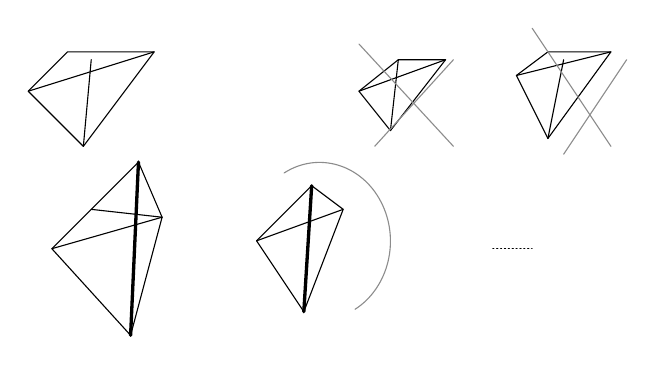
\begin{tikzpicture}[x=1mm,y=1mm,line cap=round,line join=round,font=\scriptsize]
\draw (16,-13) -- (21,-8) -- (32,-8) -- (23,-20) -- cycle;
\draw (16,-13) -- (32,-8);
\draw (24,-9) -- (23,-20);
\draw (58,-13) -- (63,-9) -- (69,-9) -- (62,-18) -- cycle;
\draw (58,-13) -- (69,-9);
\draw (63,-9) -- (62,-18);
\draw[pencil] (58,-7) -- (70,-20);
\draw[pencil] (70,-9) -- (60,-20);
\draw (78,-11) -- (82,-8) -- (90,-8) -- (82,-19) -- cycle;
\draw (78,-11) -- (90,-8);
\draw (84,-9) -- (82,-19);
\draw[pencil] (80,-5) -- (90,-20);
\draw[pencil] (92,-9) -- (84,-21);
\draw (19,-33) -- (30,-22) -- (33,-29) -- (29,-44) -- cycle;
\draw (19,-33) -- (33,-29);
\draw[very thick] (30,-22) -- (29,-44);
\draw (24,-28) -- (33,-29);
\draw (45,-32) -- (52,-25) -- (56,-28) -- (51,-41) -- cycle;
\draw (45,-32) -- (56,-28);
\draw[very thick] (52,-25) -- (51,-41);
\draw[pencil] (57.5,-40.7) arc[start angle=-60, end angle=120, x radius=9, y radius=10];
\draw[densely dotted] (75,-33) -- (80,-33);
\end{tikzpicture}
\end{document}
